Suppose the following are given:
\begin{enumerate}
	\item counter-constant columns \target{} and $\target{}\new{}$,
	\item binary columns $\bit{1}$ and $\bit{2}$,
	\item a byte colunm \target\byte{},
	\item a counter-constant column \target\mark{},
	\item a counter-constant column \size{},
	\item an accumulator column \ACC{},
	\item a ``powers of 256 column'' column \col{P},
	\item a ``counter column'' \ct{}.
\end{enumerate}
The interpretation is as follows:
\target{} is a counter-constant column containing a value from which we wish to remove a chunk of consecutive bytes;
\target\byte{} is \target{}'s byte decomposition;
$\target{}\new{}$ is the counter-constant column that will contain the result of excision;
\target\mark{} is a byte marker in \target{};
\size{} is the number of bytes to remove from \target{} starting at byte offset \target\mark{};
we expect $\target\mark{} + (\size{}-1) \leq \llargeMO$;
$\bit{1}$ plateaus at \target\mark{}, $\bit{2}$ plateaus at $\target\mark{} + \size{}$;
the bytes to be excised are accumulated in \ACC{};
\col{P} is a ``powers of 256 column'' pegged to $\bit{2}$.

We collect the following constraints under the moniker $\excision{}$:
\begin{enumerate}
	\item plateau constraints:
		\begin{enumerate}
			\item $\plateau(\bit{1}, \target{}\mark{}; \ct{})$
			\item $\plateau(\bit{2}, \target{}\mark{} + \size{}; \ct{})$
		\end{enumerate}
	\item chunk constraint: $\compChunk(\ACC{}, \target{}\byte{}, \bit{1}, \bit{2}; \ct{})$;
	\item power constraint: $\power(\col{P}, \bit{2}; \ct{})$
	\item value enforcement:
		\[
			\If
			\ct_i = \llargeMO~
			\Then
			\target\new_i = 
			\target_i - \ACC{}_i\cdot\col{P}_i
		\]
\end{enumerate}
We subsume this collection of constraints under the moniker
\[
	\excision
	\left( \begin{array}{c}
		\target{}, \target{}\new{}; \target{}\byte{};
		\acc{1}, \pow{1}; \\
		\tbo{}, \size{};
		\bit{1}, \bit{2}; \ct{};
	\end{array} \right)
\]

\begin{figure}[h!]
	\centering
	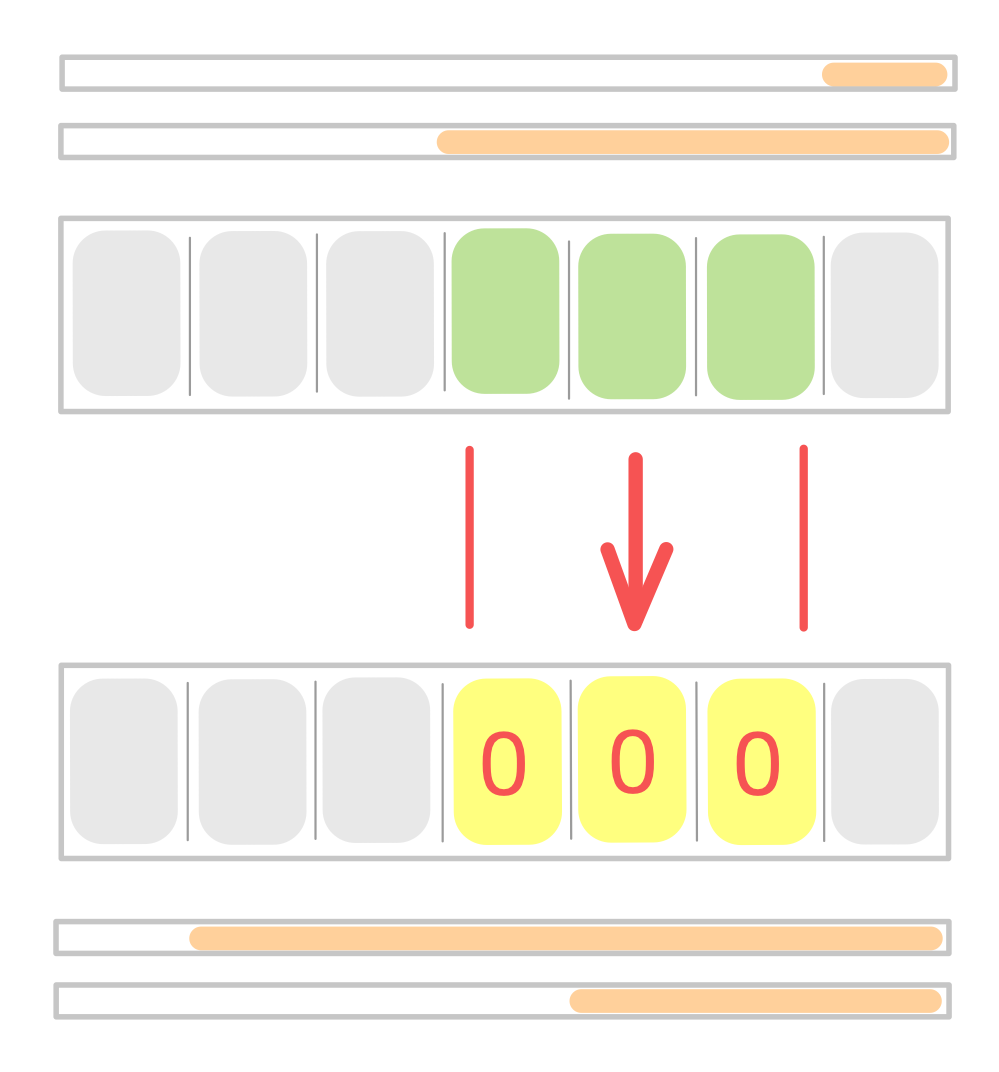
\includegraphics[width = 0.4\textwidth]{drawing/excision}
	\label{fig: one partial to one padded}
	\caption{Representation of the constraints implemented by $\excision$.}
\end{figure}
